\documentclass{article}
\usepackage{geometry}
\usepackage{paralist}
\usepackage[T1]{fontenc}
\usepackage{reledmac}
\usepackage{changepage}
\usepackage{amsmath}
\usepackage{scalerel,amssymb}
\usepackage{colortbl}

\usepackage{pgfplots}
\usepackage{tikz}
\usetikzlibrary{positioning}
\usetikzlibrary{shapes.geometric, arrows}
\tikzstyle{arrow} = [thick,->,>=stealth]

\graphicspath{ {./image/} }

\usepackage{fancyhdr}
\fancyhead[L]{
	\begin{tabular}{l}
		\LARGE \textbf{\textsc{Cryptographic Protocols}} \\
		\large Exercise 02
	\end{tabular}
}
\fancyhead[R]{
	\begin{tabular}{r}
		16-124-836 \\
		Marcel \textsc{Zauder}
	\end{tabular}
}
\renewcommand{\headrulewidth}{0.4pt}
\fancyfoot[C]{\thepage}
\renewcommand{\footrulewidth}{0.4pt}

\usepackage{hyperref}

\begin{document}
	\pagestyle{fancy}
	\hfill
	
	\section*{2.1 Circuit for comparing two numbers}
	\begin{adjustwidth}{2em}{2em}
		\subsection*{1.1.1 Algorithm for which number is bigger}
		\begin{adjustwidth}{2em}{}
			The modified algorithm, for evaluating if a number $x$ is bigger than a number $y$, with:
			\[
				[x]_2 \ = \ x_{n-1}x_{n-2}...x_1x_0 $$$$
				[y]_2 \ = \ y_{n-1}y_{n-2}...y_1y_0
			\]
			, can look like the following:
			\begin{align*}
				& i \leftarrow n \\
				& b_x \leftarrow 1 \\
				& b_y \leftarrow 1 \\
				& I \leftarrow 0 \\
				& \textit{while } i \ \geq \ 0 \textit{ do} \\
				& \ \ \ i \leftarrow i-1 \\
				& \ \ \ \textit{if } (x_i \oplus y_i) \\
				& \ \ \ \ \ \ \textit{if } (x_i \wedge \neg I) \\
				& \ \ \ \ \ \ \ \ \ b_x \leftarrow 1 \\
				& \ \ \ \ \ \ \ \ \ b_y \leftarrow 0 \\
				& \ \ \ \ \ \ \ \ \ I \leftarrow 1 \\
				& \ \ \ \ \ \ \textit{else if } (y_i \wedge \neg I) \\
				& \ \ \ \ \ \ \ \ \ b_x \leftarrow 0 \\
				& \ \ \ \ \ \ \ \ \ b_y \leftarrow 1 \\
				& \ \ \ \ \ \ \ \ \ I \leftarrow 1 \\
				& \textit{return } (b_x, b_y)
			\end{align*}
			This algorithm searches for difference in the bitsequence of $x$ and $y$. If there is a difference, the corresponding "indicate value" ($b_x, b_y$), will be set to $1$ and the other to $0$. Because we have a binary number the highest $1$ bit is decisive to which value is bigger, therefore the "indication bit" $I$ is needed so when $b_x, b_y$ were overwritten it does not need to change them again.
		\end{adjustwidth}
		\subsection*{1.1.2 Describe the corresponding circuit.}
		\begin{adjustwidth}{2em}{}
			First we are checking if $x_i$ and $y_i$ differ. In that case the indication bit $I$ is set to 1, therefore it blocks any new differences which will occur in a later, less significant bit pair. In the lower part of the diagram the signals only come through if the two bits were different and the $I$ was 0. There the values would be overwritten according to which value was higher. In the end the values of $b_x$ and $b_y$ are returned; $I$ is discarded. \\ \\
			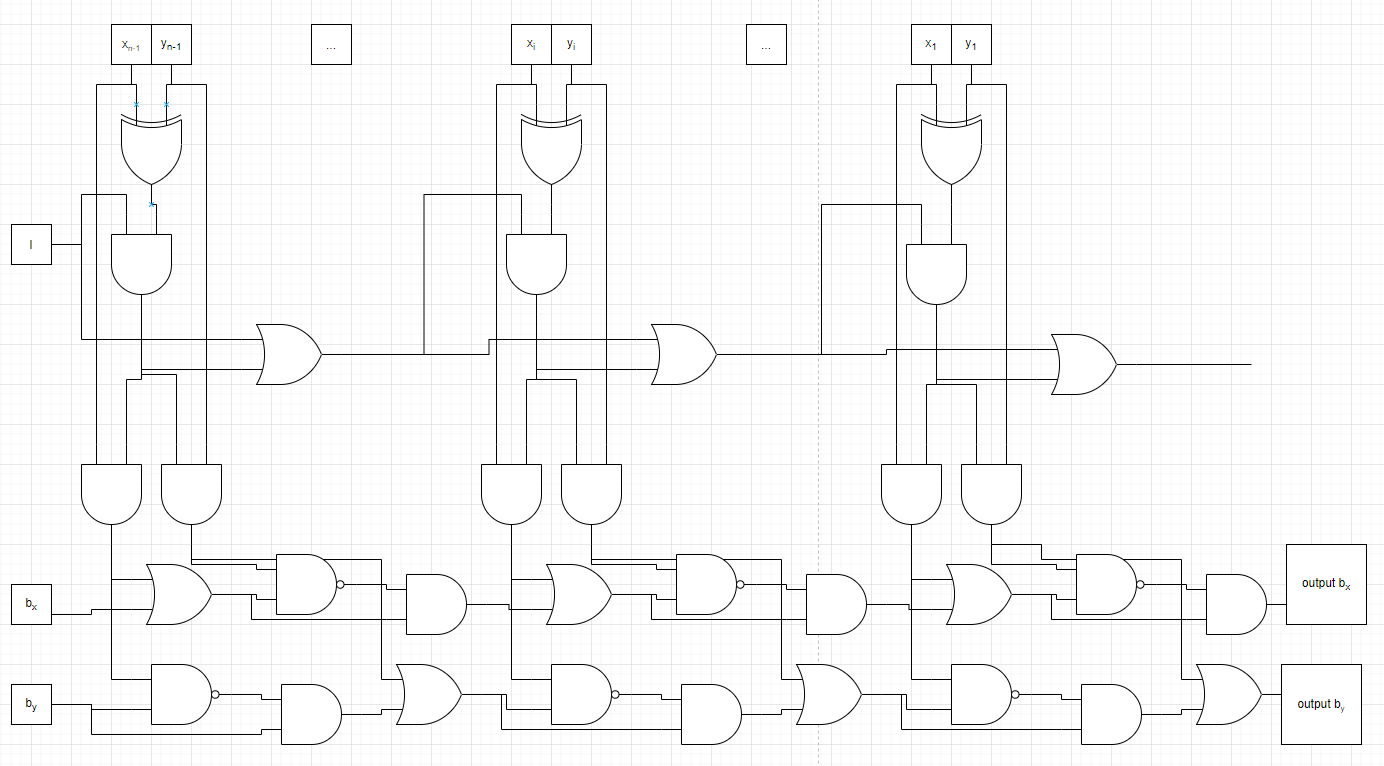
\includegraphics[scale=0.35]{Circuit_Diagram}
		\end{adjustwidth}
	\end{adjustwidth}
	
	\section*{1.2 Homomorphic Encryption}
	\begin{adjustwidth}{2em}{2em}
		\[
			\textsc{Enc}(pk, m_1) \otimes \textsc{Enc}(pk, m_2) \ = \ \textsc{Enc}(pk, m_1 \oplus m_2)
		\]
		\subsection*{1.2.1 ElGamal Encryption Scheme (Textbook)}
		The encoding process looks as follows:
		\[
			Enc(pk, m) \ = \ (g^{r}, m \cdot Y^{r})
		\]
		For $m_1$ and $m_2$ we then get:
		\begin{align*}
			Enc(pk, m_1) \ & = \ (g^{r_1}, m_1 \cdot Y^{r_1}) \\
			Enc(pk, m_2) \ & = \ (g^{r_2}, m_2 \cdot Y^{r_2})
		\end{align*}
		For the operations $\otimes$ and $\oplus$ we then get:
		\begin{align*}
			Enc(pk, m_1) \ \otimes \ Enc(pk, m_2) \ & = \ (g^{r_1}, m_1 \cdot Y^{r_1}) \ \otimes \ (g^{r_2}, m_2 \cdot Y^{r_2}) \\
			& = \ (g^{r_1} \ \otimes \ g^{r_2}, m_1 \cdot Y^{r_1} \ \otimes \ m_2 \cdot Y^{r_2}) \\
			The \ \otimes \ can \ be \ replaced &\ with \ a \ multiplication \ (\cdot): \\
			& = \ (g^{r_1} \ \cdot \ g^{r_2}, m_1 \cdot Y^{r_1} \ \cdot \ m_2 \cdot Y^{r_2}) \\
			& = \ (g^{r_1 + r_2}, \underbrace{m_1 \ \cdot \ m_2}_{m_3} \cdot Y^{r_1 + r_2}) \\
			& = \ Enc(pk, m_3) & with \ m_3 \ = \ m_1 \cdot m_2
		\end{align*}
		\subsection*{1.2.2 RSA Encryption Scheme (Textbook)}
		The encoding process looks as follows:
		\[
			Enc(pk, m) \ := \ m^{pk} \ \% N
		\]
		For $m_1$ and $m_2$ we then get:
		\begin{align*}
			Enc(pk, m_1) \ & = \ m_1^{pk} \ \% N \\
			Enc(pk, m_2) \ & = \ m_2^{pk} \ \% N
		\end{align*}
		For the operations $\otimes$ and $\oplus$ we then get:
		\begin{align*}
			Enc(pk, m_1) \ \otimes \ Enc(pk, m_2) \ & = \ m_1^{pk} \ \% N \ \otimes \ m_2^{pk} \ \% N \\
			& = \ (m_1^{pk} \otimes m_2^{pk}) \ \% N \\
			The \ \otimes \ can \ be \ replaced &\ with \ a \ multiplication \ (\cdot): \\
			& = \ (m_1^{pk} \cdot m_2^{pk}) \ \% N \\
			& = \ ((\underbrace{m_1\cdot m_2}_{m_3})^{pk}) \ \% N \\
			& = \ Enc(pk, m_3) & with \ m_3 \ = \ m_1 \cdot m_2
		\end{align*}
	\end{adjustwidth}
\end{document}